%
% fig-2d.tex
%
% (c) 2025 Prof Dr Andreas Müller
%
\begin{figure}
\centering
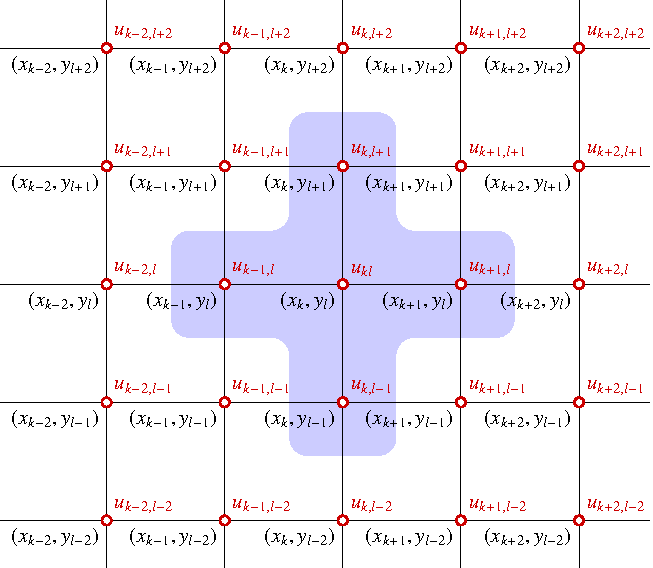
\includegraphics{chapters/090-pdenumerik/images/2d.pdf}
\caption{Diskretisation mit finiten Differenzen in zwei Dimension.
Für jeden Gitterpunkt wird einen Variable ({\color{darkred}rot}) benötigt.
Für die Berechnung einer Approximation des Laplace-Operators an der
Stelle $(x_k,y_l)$ sind die Variablen im blauen Kreuz notwendig.
\label{buch:pdenumerik:fdm:fig:2d}}
\end{figure}
